
\documentclass[useAMS,usenatbib]{mn2e}
%\documentclass[usenatbib]{mn2e}
\usepackage{graphicx}
%\usepackage[nottoc]{tocbibind}

% If your system does not have the AMS fonts version 2.0 installed, then
% remove the useAMS option.
%
% useAMS allows you to obtain upright Greek characters.
% e.g. \umu, \upi etc.  See the section on "Upright Greek characters" in
% this guide for further information.
%
% If you are using AMS 2.0 fonts, bold math letters/symbols are available
% at a larger range of sizes for NFSS release 1 and 2 (using \boldmath or
% preferably \bmath).
%
% The usenatbib command allows the use of Patrick Daly's natbib.sty for
% cross-referencing.
%
% If you wish to typeset the paper in Times font (if you do not have the
% PostScript Type 1 Computer Modern fonts you will need to do this to get
% smoother fonts in a PDF file) then uncomment the next line
% \usepackage{Times}

%%%%% AUTHORS - PLACE YOUR OWN MACROS HERE %%%%%

% Journal definitions
\newcommand{\apj}[1]{ApJ}
\newcommand{\mnras}[1]{MNRAS}
\newcommand{\apjl}[1]{ApJL}
\newcommand{\pasj}[1]{PASJ}
\newcommand{\aj}[1]{AJ}
\newcommand{\nat}[1]{Nature}

%%%%%%%%%%%%%%%%%%%%%%%%%%%%%%%%%%%%%%%%%%%%%%%%

\title[Beware the Effect of Edge-on Disks]{Gravitational Lens Modelling of Flux Ratio Anomalous System B1555+375}
\author[Hsueh et al.]{Jen-Wei Hsueh$^{1}$\thanks{E-mail:
email@address (AVR); otheremail@otheraddress (ANO)} and A. N.
Other$^{2}$\\
$^{1}$Physics Dept., University of California, Davis, 1 Shields Ave.
Davis, CA 95616, USA\\
$^{2}$Building, Institute, Street Address, City, Code, Country}
\begin{document}

%\date{Accepted 1988 December 15. Received 1988 December 14; in original form 1988 October 11}

\pagerange{\pageref{firstpage}--\pageref{lastpage}} \pubyear{2015}

\maketitle

\label{firstpage}

\begin{abstract}

Gravitational lens flux-ratio anomalies provide a powerful technique
for detecting the presence of dark matter substructure in distant
galaxies.  However, before using the statistics of systems with these
anomalies, it is imperative to ascertain that a given system does not
have properties that could plausibly cause the observed anomaly
without the need for substructure.  In this letter, we present the
case of the B1555+375 lens system, which has a strong radio-wavelength
flux-ratio anomaly but where the lensing galaxy is also revealed in
high-resolution imaging to have a clear edge-on disk component.  The
disk crosses directly over the pair of images that exhibit the
anomaly, and we show that simple models that include the disk can
reproduce the anomaly without requiring substructure.  Several [??]
other lens systems that we have observed with adaptive optics imaging
as part of the Strong lensing at High Angular Resolution Programme (SHARP)
show similar behaviour.  These results suggest that the assumption that
all flux-ratio anomalies are due to substructure will likely overestimate
the substructure fraction in massive galaxies.

\end{abstract}

\begin{keywords}
gravitational lensing
\end{keywords}

\section{Introduction}

A common feature of simulations of structure formation is the presence
of thousands of subhaloes that are associated with larger mass haloes.
However, observations of the Local Group find many fewer satellite
galaxies than are predicted by the simulations, even when taking into
account completeness corrections arising from the limited sky coverage
imposed by the Galactic Plane.  This is the famous ``missing
satellite'' problem \citep{Klypin1999, Moore1999, S07}. In order to
understand this discrepancy, it is imperative to build up a large
sample of satellites/subhaloes in galaxies outside the Local Group.
This process is challenging due to the faintness of the satellite
galaxies.  Furthermore, lower-mass satellites may not be able to
retain the gas needed for ongoing star formation \citep[e.g.,][]{P11},
rendering them effectively dark.  These factors make gravitational
lensing a powerful and promising tool for the detection of
substructure.

It was first suggested by \citet{Mao1998} that flux ratio anomalies observed in radio loud multiple images of lensed quasar could be interpreted as the telltale of the presence of substructure in lens galaxies.
%Flux ratio anomalies are seen in strong lensing systems which have multiple images that are spacially close to each other. These ``merging doubles'' share the same surface brightness in principle but happend to have different surface brightness. 
Indeed, small perturbations in the gravitational potential are
sufficient to bring flux ratio anomalies in strong lensed systems.
Moreover, unlike in the optical or infrared, in the radio band, lensed
images are not sensitive to micro lensing from stars nor dust
extinction.  This makes flux ratio anomalies a promising tool to
detect dark matter substructures \citep{Dalal2002, N13}.  At present,
the amount of substructure derived from flux ratio anomalies is in
disagreement with predictions from numerical simulations, with the
former requiring a larger fraction of mass in substructure than
expected \citet{Xu14}. While this could be the result of small sample
statistics, it could also be the indication that flux ratio anomalies
have a different origin than substructure. 

An alternative method for
the detection of substructure in gravitational lens galaxies based on
the surface brightness distribution of extended arcs and Einstein ring
has been introduced by \citet{K05,V09}. Interestingly, the fraction of
substructure measured with this \emph{gravitational imaging technique}
is currently in agreement with theoretical expectations \citep{V14a}.

While future large-scale surveys, such as the LSST, are expected to
deliver new large samples of gravitationally lensed quasars, in the
near future the discovery of new systems using narrow-line quasar
emission \citep{N14} will provide new invaluable statistical
perspective on current constraints based on flux ratio anomalies.  In
this paper, we explore the alternative idea that flux ratio anomalies
are not related to the presence of substructure but originate in a
more complex lens galaxy mass distribution than initially
considered. To this end we use new infra-red data from the Strong
lensing at High Angular Resolution Program(SHARP). The main goal of
the SHARP project is to re-observe known quadruple and Einstein ring
lens systems at a much higher angular resolution by making use of the
Keck adaptive optics (AO) telescope and large interferometric arrays
\citep{SHARP12,V12} . In particular, to better understand the cause of
flux ratio anomalies in strong lens systems we focus on the lens
modelling of the lens system B1555+375 (included in both the
observational and theoretical analysis of \citet{Dalal2002} and
\citet{Xu14}, respectively) by making use of the new information
obtained from the latest SHARP infrared imaging. The paper is
organized as follows: the latest SHARP data is introduced in section
2; in section 3 we present the lens model while the results of this
analysis and their implication are discussed in section 4.

%However, only small number of flux ratio anomalous systems in \simona{the} radio are \simona{currently} avaliable. Besides waiting for future large-scale survey such as LSST to find thousands of more new lens galaxies, another approach \simona{is to} seek out more flux ratio anomalous systems \simona{using} narrow-line quasar emission \citep{N14}. 
%	With expected growth in the number of samples, several groups have developed the technique to estimate the properties of substructures from flux ratio anomalous systems. \citet{V09, H13} both analyze the strong lens imaging to detect substructures lie infront of Einstein ring. Their methods improve the detectable mass limit and also show that high spatial resolution imaging is essential for the substructure study. On the other hand, numerical simulations on structure formation do not reach the concise conclusion on flux ratio anomalous systems. The latest study on the cause of flux anomalies from \citet{Xu14} shows the low probability of the existence of substructures in their studied systems. 
%	The Strong lensing at High Angular Resolution Program(SHARP) is a project aims on known quadruple and Einstein ring lensing systems \citep{SHARP12}. We obtain high-resoltion images from Keck adaptive optics(AO) and Hubble Space Telescope(HST) observations. 
%To better understand the cause of flux ratio anomaly in strong lensing systems, we model B1555+375, one of the systems discussed in \citet{Xu14}, with the new information obtained from the latest SHARP infrared imaging. We present the latest SHARP data in part 2, lens model of B1555+375 in part 3, and discussion in part 4. 

\section{Data Collection \& Reduction}

\begin{figure*}
%\begin{minipage}{140mm}
%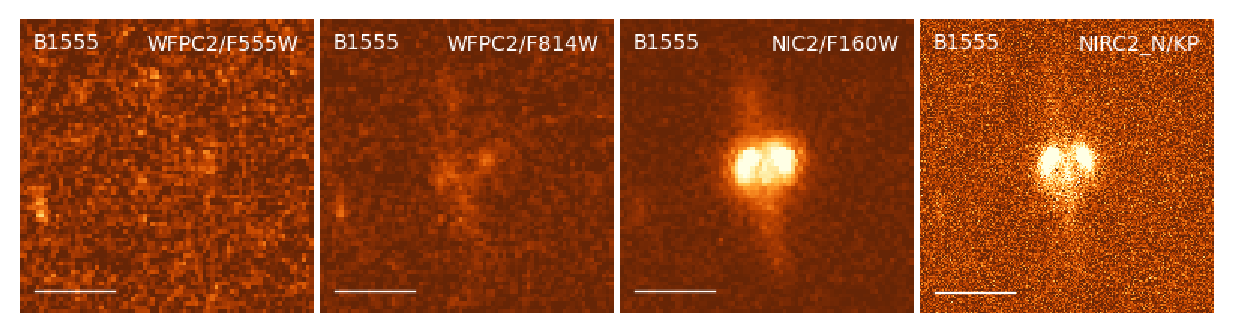
\includegraphics[width=140mm]{B1555_gallery.eps}
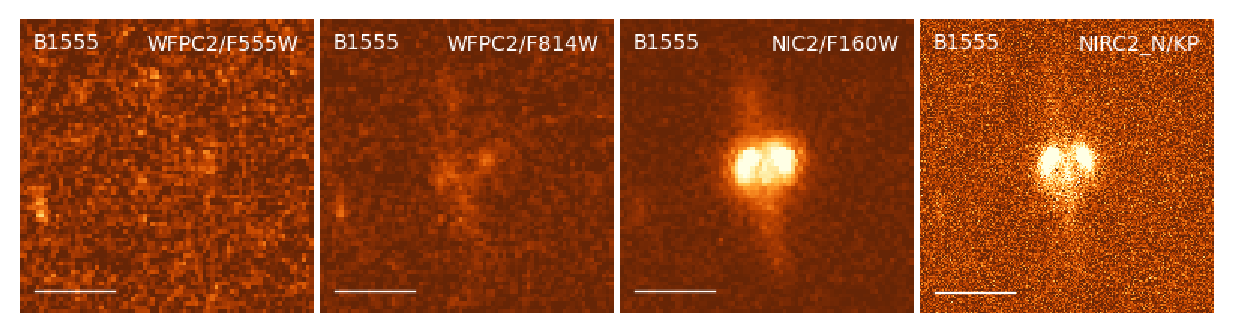
\includegraphics[width=0.95\textwidth]{B1555_gallery.eps}
\caption{High-resolution multiband imaging of the B1555+375 lens system.
All of the panels are 3\farcs7 on a side, and for each panel the scale bar 
represents 1\arcsec.  From left to right the figures show data from
HST/WFPC2 in the F555W band, HST/WFPC2 in the F814W band, HST/NICMOS/NIC2
in the F160W band, and Keck AO imaging in the $K^\prime$ band.
\label{fig:multiband}}
%
%\end{minipage}

\end{figure*}

\subsection{Keck Adaptive Optics Imaging}

The B1555+375 system was observed using the NIRC2 camera on the Keck 2
Telescope on the night of 2012 May 16 UT.  The adaptive optics system
was used, with the corrections derived from the laser guide star and a
$R$=14.4 tip-tilt that was located 45$^{\prime\prime}$ from the lens
system.  The ``narrow camera'' mode was used, giving a field of view
of roughly 10$^{\prime\prime}$\ on a side and a pixel scale of 10~mas.
Six dithered 300~s exposures were obtained in $K^{\prime}$ band.  The
data were reduced with the standard SHARP pipeline, which is a
python-based package that is a refinement of the process described in
\citet{Auger_EELS1}.  A cutout of the final reduced image is shown in
Fig.~\ref{fig:multiband} and again in Fig.~\ref{fig:merlin} with
contours from the MERLIN radio observations of \citet{Marlow}
overlaid.  There are several notable features in the Keck AO data.
These include the nearly complete lack of emission associated with the
B and D lensed images, as can be seen by comparing the radio contours
to the $K^\prime$-band emission, and faint but clearly visible
emission from what appears to be an edge-on lensing galaxy.

\subsection{Hubble Space Telescope Archival Imaging}

The B1555+375 system was also observed by the Hubble Space Telescope
(HST) in three broad bands.  The optical data were obtained with the
Wide-Field Planetary Camera 2 (WFPC2) in the F555W and F814W bands
(GO-8804; PI: E.\ Falco), while the Near Infrared Multi-Object
Spectrograph (NICMOS) was used to observe the system in the $F160W$
band (GO-9744; PI: C.\ Kochanek).  The NICMOS observations were
obtained with the NIC2 camera.  We reduced all of the archival HST
data with the standard {\tt multidrizzle} pipeline [?? CHECK WITH
  MATT], producing final drizzled images with pixel scales of 50~mas.
The reduced images are shown in Figure~\ref{fig:multiband}.  The lens
system is not detected at high significance in the optical bands, but
is clearly seen in the NICMOS $F160W$ image.  The edge-on lensing
galaxy stands out in the NICMOS image.

The observation details of Keck AO and HST imaging are shown in Table 1.

\begin{table}
 \centering
 %\begin{minipage}{140mm}
  \caption{Multiband observation details of the B1555+375 lens system.}
  \begin{tabular}{@{}llccc}
  
\hline
  Telescope     &      Camera     &  Band & Date &$t_{exp}$ (s) \\

 \hline
   HST				&		WFPC2    &  F555W		&	2000/10/09 	&	5200\\
   HST				&		WFPC2    &  F814W		&	2000/10/09 &	5200\\
   HST				&		NICMOS/NIC2	&	F160W	&	2003/11/02 & 5376\\
   Keck2			&		NIRC2 AO	&   $K^\prime$	& 2012/05/16	&  1800\\
   \hline
\end{tabular}
%\end{minipage}
\end{table}

%===========================================================================

\section{Lens Modelling}

To model B1555+375, we use the lens modeling code {\tt glafic}
\citep{Oguri}.  The inputs to the model are the observed image
positions and flux densities measured by the radio observations of
\citet{Marlow}.  These authors present a singular isothermal ellipsoid
(SIE) model that provides the first fit to the image positions but
does not reproduce the strong flux ratio anomaly between components A
and B.  \citep[see Fig.~6 and Tables 2 \& 3 in][]{Marlow}.  Although
the flux ratio anomaly that is observed in the radio data may be
caused by substructure in the lensing galaxy, our high-resolution near
infrared imaging suggests another explanation.  In both the $K^\prime$
band adaptive optics data and the HST imaging (two rightmost panels in
Fig. 1), the lensing galaxy has a clear edge-on disk component with a
position angle of $\approx 10$ degree.  We therefore model the system
with a disk component in order to see if such a model can explain the
flux ratio anomaly without the need for substructure.  The edge on
disk may also explain the system morphology that is observed in the
near infrared imaging.  In particular, neither image B nor image D is
detected in the Keck AO data (Fig.~\ref{fig:merlin}), and both of
these lensed images lie on or close to the edge-on disk.  Thus, strong
extinction in the disk could cause the lack of detection of these
images.

We have created two separate models of the lensing potential.  In the
first we treat the lens as a SIE bulge and an exponential edge-on disk
(SIE+expdisk).  In the second model the disk is represented as a very
elongated SIE component (2-SIE).  The lens system is red, with a
strong jump in flux between the F814W (roughly I) and F160W (roughly
H) bands (Fig.~\ref{fig:multiband}), so we assign a lens redshift of
$z_\ell = 1.0$ and a source redshift of $z_s =1.5$.  The full best-fit parameters are shown in Table
2. Both of these models predict fairly matched results with the radio
observation, and the 2-SIE model has a better performance in flux
ratios. The comparison of observation and our lens modelling is given
in Figure 3 and Tables 3 \& 4.

\begin{figure}
%\plotone{1555_ao_merlin_overlay.eps}
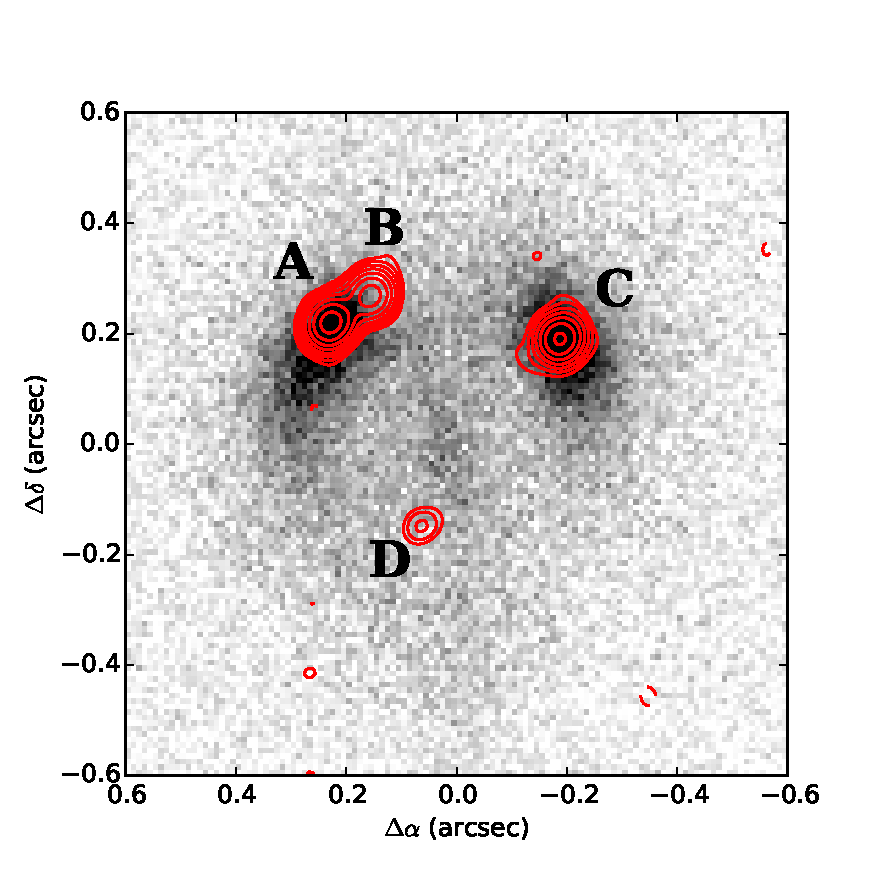
\includegraphics[width=84mm]{1555_ao_merlin_overlay.eps}
\caption{High-resolution  $K^\prime$ band imaging of the B1555+375 lens system 
with contours from the MERLIN observation of \citet{Marlow} overlaid.
%
\label{fig:merlin}}
\end{figure}


\begin{figure}
%\plotone{point_source.eps}
\includegraphics[width=84mm]{point_source.eps}
\caption{Radio observation(red open circle) and model-predicted(blue plus sign) image positions of B1555+375. The position of the source is at $(-0.2066,-0.1634)$ for SIE+Expdisk model, marked by a black filled circle. From left to right, four components are A, B (merging doubles), D(lowest spot), and C(right).\label{fig2}}
\end{figure}



\begin{table}
% \centering
% \begin{minipage}{140mm}
  \caption{Best-fit parameters of B1555+375 lens model.}
  \begin{tabular}{@{}ccc}
\hline 
 Parameter  & \multicolumn{2}{c}{Lens model} \\
		&SIE+expdisk& 2-SIE		   
\\
\hline
$x_1$  	& $-0.1883$	& $-0.1809$	  \\
$y_1$	&$-0.1923$	&$-0.1702$	  \\
$x_2$	&$-0.1615$ 	&$-0.1592$	  \\
$y_2$	&$-0.2502$	& $-0.1833$	  \\
$\sigma_1$	&$141.3$ &	$144.6$	  \\
$M_{tot} / \sigma_2$& $3.59\times 10^{10} $  &$123.8$ 	 \\  
$e_1$	& $0.27$	& $0.27$ \\  
$\theta_1$	&$105.5 \degr$ & $97.7 \degr$	 \\
$e_2$	&$0.84$	&$0.83$      \\
$\theta_2$	&$7.4\degr$ &$7.4\degr$  \\
$r_e$	& $0.20 ''$ &  -- \\
\hline
\end{tabular}

%\end{minipage}
\medskip
Subscripts 1 and 2 represent bulge and disk components in each model respectively. Positions are offsets from radio image component A measured in units of arcsec. The velocity dispersion $\sigma$ is in units of $km/s$ and disk mass $M_{tot}$ is in units of $h^{-1} M_{\odot}$. $e$ is ellipticity and $\theta$ is the position angle measured east of north.

\end{table}

\begin{table*}
%\centering
 \begin{minipage}{140mm}
  \caption{Radio observation and model-predicted lensed image positions.}
  \begin{tabular}{@{}ccccccc}

\hline

Component	&\multicolumn{2}{c}{MERLIN} 	 & \multicolumn{4}{c}{Model} \\
					&\multicolumn{2}{c}{5 GHz}		&	\multicolumn{2}{c}{SIE+expdisk} &\multicolumn{2}{c}{ 2-SIE}		\\
					 &East &North &East 		&North &East 		&North\\ 
\hline
A ........ &$0$    		&$0$		&$0.0000$ &$0.0000$   &   $0.0000$   &  $ 0.0000$\\  
B ........ &$-0.0726$ 	&$+0.0480$	&$-0.0726$ &$+0.0479$ & $-0.0726 $  &  $+0.0480$  \\  
C ........ &$-0.4117$  &$-0.0280$	&$-0.4117$ &$-0.0280$  & $-0.4117 $  &   $+0.0280$ \\  
D ........ &$-0.1619$  &$-0.3680$	&$-0.1609$ &$-0.3678$  & $-0.1618$    &  $+0.3680$ \\  
\hline
\end{tabular}

\end{minipage}
\medskip

Comparision between radio and model-predicted lensed image positions. Observation data quoted from Table 2 in \citet{Marlow}. Position offsets are in unit of arcsec. Both SIE+expdisk and 2-SIE lens model-predicted positions well match to the radio observation.

\end{table*}

\begin{table}
% \centering
% \begin{minipage}{140mm}
  \caption{Flux ratios of B1555+375 components.}
  \begin{tabular}{@{}ccccccc}

\hline
	& MERLIN & VLA & \multicolumn{3}{l}{Model}\\
		&5 GHz & 15 GHz  & 1-SIE & SIE+expdisk & 2-SIE\\
\hline
$f_A/f_B$			&$1.75$ & $1.78$ &$1.07$& $1.66$ & $1.75$ \\ 
$f_A/f_C$		&$2.05$ 	&$2.37$ &$2.95$ & $1.33$ & $2.16$\\
$f_A/f_D$		&$13.08$ &$ 12.86$ &$2.00$& $5.83$ & $7.96$\\

\hline
\end{tabular}

%\end{minipage}
\medskip
Comparision between radio data and model-predicted flux ratios. Radio observation data is quoted from Table 2 and Table 3 in \citet{Marlow}. 1-SIE model is quoted from Tabel 5 in \citet{Marlow}.

\end{table}

\section{Discussion}

We present new lens models of B1555+375. With the new imaging from SHARP $K^{\prime}$ band, the most significant difference comparing to previous modelling is a new edge-on disk component. With a bulge plus an edge-on disk, our models fairly match to the radio image positions and also flux ratio anomalies, while models with only one SIE component \citep{Marlow,Xu14} fail. Radio propagation effects are ruled out in B1555+375 \citep{K03,KD04}. Our successful modelling indicates that the structure from lens galaxy itself causes the flux ratio anomalies in B1555+375. An edge-on disk with high ellipcity well explains the observed flux ratios without the presense of substructrues. This breaks the idea that in strongly lensed quasars, radio flux ratio anomalies are most likely originated from substructure perturbations. It is worth noticing not all of flux ratio anomalies in lensed quasars indicate the existence of substructures. Our discovery shows a complex lens galaxy mass distribution can dominate flux ratio anomalous phenomena in a strongly lensed system. 

The abundance of substructures within galaxy-size haloes has been an undetermined problem in structure formation studies. Discrepencies between numerical simulations and observations within the local universe gives two possible interpretations: an alternative structure formation model or a small sample set from nowaday observations. Difficulties emerge in direct detection when searching beyond the Local Group. Until now, most of known satellites are at high mass end in the mass function. However, the gravitational perturbation from substructures can cause detectable change in surface brightness among lensed images. This makes gravitational lensing a powerful tool for searching substructures. Flux ratio anomalies in strongly lensed quasars become a sign of existence of subhaloes. Total mass of substructures can be derived from their gravitational effects and also give direct measurement of mass function, avoid making assumptions on baryonic matter distribution assoociated with dark matter.

Given the assumption that lens galaxy has smooth gravitational potential, only substructure perturbations can cause flux ratio anomalies (in ideal case, i.e. no dust extinction, micro lensing, scattering etc.). Numerical simulations demostrate this idea with known flux anomalous lensed quasars. In \citet{Xu14}, they found that substructures cannot expalin all radio flux anomalies. By adding subhaloes on to those systems, only one out of six lens systems reproduces the flux anomalies. The rest of them are unlikely to have substructure originated flux anomalies, including our target B1555+375. \citet{Xu14} conclude the failure on B1555+375 is due to improper lens models. This result supports our discovery in both observation and lens modelling, that an edge-on disk lies  between the radio merging double explain its flux ratio anomaly. 

From the successful modelling of B1555+375,  we expect more flux anomalous systems requiring complex lens models (e.g. include an exponential disk), rather than just assuming smooth potential. Although the number of radio loud flux anomalous lensed quasars remains small, a new technique using narrow-line emissions will enlarge the sample and bring statistical perspective on substructures in the near future \citep{N14}. If the non-substructure effect from edge-on disks does not included, expected ``false'' substructure detections can serverly bias the data analysis. Even with real substructures presence, the lens galaxy structure can still dominate flux anomalous phenomena. For precise measurements on substurcture population, mass function, and any derived properties from strongly lensed flux anomalous systems, it is crucial to have careful estimation on non-substructure effects. We would like to draw attention to this edge-on disk orginated flux anomalies due to its impacts on substructure searching.

Our results also demostrate that multi-wavelength imaging is helpful to explore flux anomalous lensed quasars. Although radio band provides reliable data on positions and fluxes of lensed images, optical and near-infrared imaging provides more information on mass distribution of the lens galaxy. In the previous paper of SHARP, \citet{SHARP12} show that high resolution IR imaging can help to improve lens modelling. The improvement is even more dramatic in B1555+375. With an high ellipcity edge-on disk, our new lens models adequately explain the flux ratio anomaly. Lack of knowledge of lens galaxies can lead to improper lens modelling and bias to statistics among substructure detections. With the first system analyzing and finding that an edge-on disk from the lens galaxy can dominate its flux ratio anomaly, our follow up will be explore other SHARP systems. In Figure 3, all of these systems have a recognizable edge-on disk in infrared imaging. An edge-on disk structure may also be able to expalin the flux ratio anomalies of these systems.\\
 

\section*{Acknowledgments}

\bibliographystyle{mn2e}
\bibliography{reference.bib}




\label{lastpage}

\end{document}
